% !TeX spellcheck = en_US

\chapter{Concept and Architecture}\label{chap:conarch}
In this chapter, the concept and the architecture of the software which can satisfy the requirements, presented in chapter \ref{chap:req}, will be explained and substantiated.
The chosen solution is to build a modular framework, where each module will be responsible for identification and resolution of the specific external references type.
During resolution, external data will be downloaded and integrated into the structure of the processed CSAR.
%A user will have an opportunity to choose the method of the encapsulation, the "sets of packages" or "one node for one package" which were described in section~\ref{subs:encaps}.
%Solutions to some additional problems will be presented. 
\section{Concept}
In this section, the main concept of this work are described.
The general structure of the framework is visualized in Figure~\ref{fig:gen}. 
Three types of modules will be introduces: $language$ $modules$, $package$ $manager$ $modules$ and $download$ $tool$ $modules$.
Language modules will handle configuration files written in the corresponding language.
Package manager modules and download tool modules will proceed the package installation commands and data download commands respectively.
They will identify and resolve external references and call the topology handler which will update the internal structure of TOSCA applications. \\
In section~\ref{subs:analyse}, it will be explained how to determine the Node Templates which use the given artifact.
Then functionality of language modules, package manager modules and download tool modules will be presented.
In section~\ref{subs:repres}, it will be expressed how to create a new node for a TOSCA topology. 
After that, some methods to determine the architecture of the final platform will be presented.
%In addition, it will be described, how the results can be validated.
% !TeX spellcheck = en_US

\begin{figure}
	\centering
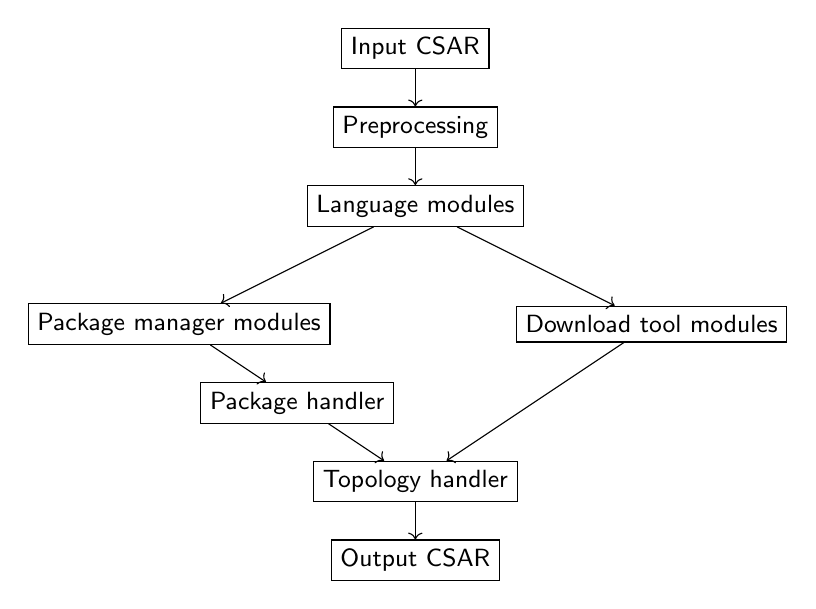
\begin{tikzpicture}
\node[draw] (in) at (0,1.5) {Input CSAR};
\node[draw] (pp) at (0,+0.5) {Preprocessing};
\node[draw] (lm) at (0,-0.5) {Language modules};
\node[draw] (pmm) at (-3,-2) {Package manager modules};
\node[draw] (dtm) at (+3,-2) {Download tool modules};
\node[draw] (ph) at (-1.5,-3) {Package handler};
\node[draw] (th) at (0,-4) {Topology handler};
\node[draw] (out) at (0,-5) {Output CSAR};
\draw [->] (in) -- (pp);
\draw [->] (pp) -- (lm);
\draw [->] (lm) -- (pmm);
\draw [->] (lm) -- (dtm);
\draw [->] (pmm) -- (ph);
\draw [->] (dtm) -- (th);
\draw [->] (ph) -- (th);
\draw [->] (th) -- (out);
\end{tikzpicture} 
\caption{The general description of the software's work flow} 	\label{fig:gen}
\end{figure}

\subsection{Analysis of a TOSCA-Topology}\label{subs:analyse}
To update the \gls{tosca} topology properly, it is necessary to add references from the nodes where external references were to the newly created nodes which resolve the external references. 
For the given artifact with an external reference, one need to find all Node Templates which use this artifact, create for each of them new Node Templates resolving the reference and define the dependencies between them.
The search can be done once for all artifacts during the preprocessing stage.
Later one can use the results of the search to identify all Node Templates for the given artifact.
%According to TOSCA standard, references between Node Templates can only be created in the same Service Template.  
%That means that each Node Template which uses artifacts with external references must be found.
Furthermore, Service Templates where these Node Templates are defined must be determined to create there new Node Templates and Relationship Templates.
The pointers to artifacts are stored in Artifact Templates which are used by Node Type Implementations.
Node Type Implementations implement Node Types wich are instantiated by Node Templates.
By composing all the information the references chain can be built:\\
$Artifact$ $\rightarrow$ $Artifact$~$Template$ $\rightarrow$ $Node$~$Type$~$Implementation$ $\rightarrow$ $Node$~$Type$ $\rightarrow$ $Node$~$Template$ $\rightarrow$ $Service$~$Template$\\
Now consider the references in more detail. 
\begin{itemize}
	\item $Artifact$ $\rightarrow$ $Artifact$ $Template$\\
	An Artifact can be referenced by several Artifact Templates. (Despite the fact that this is a bad practice.)
	\item  $Artifact$ $Template$ $\rightarrow$ $Node$ $Type$ $Implementation$ \\
	The same way an Artifact Template can be used by several Node Type Implementations.
	\item $Node$ $Type$ $Implementation$ $\rightarrow$ $Node$ $Type$ \\
	A Node Type Implementation can describe an implementation of only one Node Type.
	\item  $Node$ $Type$ $\rightarrow$ $Node$ $Template$\\
	Each Node Type can have any number of Node Templates.
	\item  $Node$ $Template$ $\rightarrow$ $Service$ $Template$\\
	But each Node Template is defined only once.
\end{itemize}
This structure can be described as a tree with an Artifact as a root and Service Templates as leaves, and will be called the internal dependencies tree.
The example is provided by Figure~\ref{fig:script_serv}.\\
%Of course it is possible to move in opposite direction, starting from a Node and moving toward scripts, but this method brings additional complexity. 
There is an additional problem in references between Node Types and Node Type Implementations.
A Node Type can have several implementations, but which one will be used is determined only during the deployment. 
The chosen solution to this problem is to use each Node Type Implementation in the hope, that they will not conflict.\\
%The method presented above can uniquely determine Node Templates and Service Template for a given script.
%Of course it is not guaranteed that found Node Type Implementation will be used during deployment, but we can't do anything with this. 
The following steps to build the internal dependencies tree can be executed during the preprocessing.
\begin{itemize}
	\item Find all Artifact Templates to build references from Artifacts to Artifact Templates.
	\item Find all Node Type Implementations. 
		Since they contain references both to the Node Type and to the Artifact Templates, the dependency from Artifacts to Node Types can be built.
	\item Find all Service Templates and all Node Templates they contain. 
		Each Node Template refers to its Node Type what is useful for building a dependency from Artifact to Node Template.
\end{itemize} 
In this way the required internal dependencies tree with references \\$Artifact$~$\rightarrow$~$Node$~$Template$ and $Artifact$~$\rightarrow$~$Service$~$Template$ can be built.
% !TeX spellcheck = en_US
\usetikzlibrary{calc,arrows.meta,positioning}
\tikzset{
    every node/.style={font=\sffamily\small},
    main node/.style={shape=rectangle, rounded corners,
    	draw, align=center,
    	top color=white, bottom color=blue!20}
}

\begin{figure}
	\centering
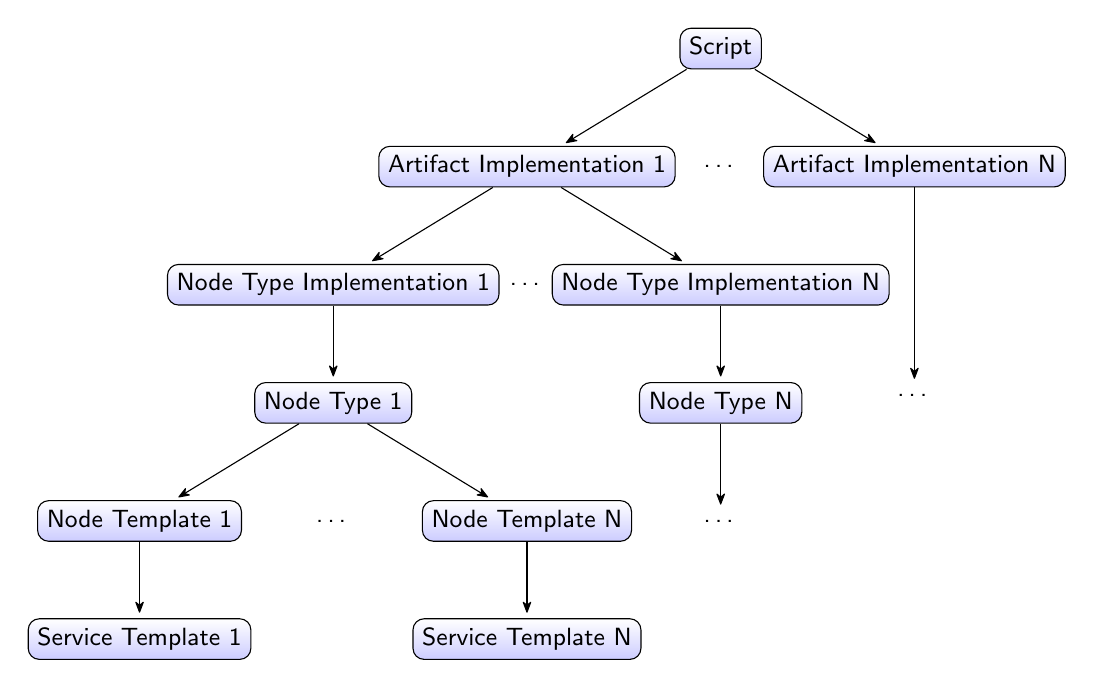
\begin{tikzpicture}[sibling distance=14em,->,>={Stealth[round,sep]},shorten >=1pt,auto,node distance=25mm]
    \node[main node] (1) {Script}
    child { node[main node](3) {Artifact Implementation 1} 
    	child { node[main node] (6) {Node Type Implementation 1} 
    			child { node[main node] (8) {Node Type 1} 
    				child { node[main node]  (11) {Node Template 1} 
    					child { node[main node] (13) {Service Template 1}}  
    				}
    				child { node[main node]  (12) {Node Template N} 
    					child { node[main node] (14) {Service Template N}}
    				}
    			}
    	}
    	child { node[main node] (7) {Node Type Implementation N} 
    		child { node[main node] (9) {Node Type N} 
    			child { node  (10) {\ldots} }
    		}
    	}
    }
    child { node[main node] (4) {Artifact Implementation N}  
    child { node (5) [below =of 4]{\ldots}}
	};

    \node at ($(3)!.5!(4)$) {\ldots};
    \node at ($(6)!.5!(7)$) {\ldots};
    \node at ($(11)!.5!(12)$) {\ldots};
    
\end{tikzpicture} 
\caption{Example tree describing how to find Service Templates and Node Templates for a given script} 	\label{fig:script_serv}
\end{figure}

\subsection{Search for Artifacts}\label{subs:searchart}
Since artifacts may contain external references, we need to find all of them in order to resolve the references.
The first simple solution is to analyze the structure of a TOSCA application and to identify all Artifact Templates and corresponding artifacts.
But this method brings possibility to miss artifacts because some of them can be called from other artifacts and may be not presented in the TOSCA topology by an Artifact Template.
This case is presented by Figure~\ref{fig:artart}.
In this example the "Artifact 1" was deployed into Database by Implementation Artifact Engine and is called by a management plan.
The "Artifact 2" is an executable file without an Artifact Template.
That is a bad practice, but we must consider that option too, to provide higher level of reliability.
It is possible, that the "Artifact 2" will not be considered by the method described above.
The found solution is to analyze all files presented in input CSARs and resolve external references in all of them.
One needs to define methods to identify configuration files for each supported configuration management tool.
% !TeX spellcheck = en_US

% We need layers to draw the block diagram
\usetikzlibrary{calc,positioning}
\usetikzlibrary{arrows.meta}

% Define a few styles and constants
\tikzstyle{entry}=[draw, minimum height=2em, align=center]
\tikzstyle{mytext}=[align=center]
\tikzstyle{frame} = [entry, text width=28em, fill=white,minimum height=10em, rounded corners]
\tikzstyle{engine} = [entry, text width=7em, fill=white,minimum height=4em, rounded corners, left color=green!15!white, right color=green!20!white,shading angle=135, anchor=north]
\tikzstyle{store} = [entry, text width=16em, fill=white,minimum height=6em, rounded corners, left color=blue!15!white, right color=blue!20!white,shading angle=135, anchor=north]
\tikzstyle{art} = [entry, text width=5em, fill=white,minimum height=3em, rounded corners, left color=red!15!white, right color=red!20!white,shading angle=135, anchor=north]
\def\blockdist{2.3}
\def\edgedist{2.5}

\begin{figure}
	\centering
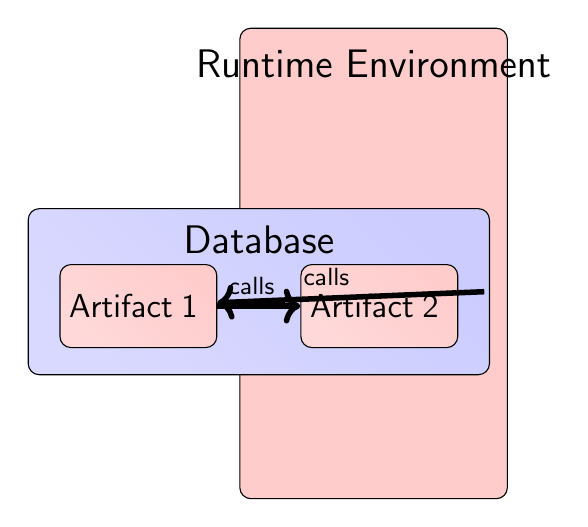
\begin{tikzpicture}
\node (frame) [frame, label={[shift={(+0ex,-5ex)}]north:{\Large Runtime Environment}}] {};

\node (engine) [xshift=+5em, yshift=+1em] at (frame.west) [engine] {\large Management plan};
\node (storage) [xshift=-9em, yshift=+2em] at (frame.east) [store,label={[yshift=-2em]north:{\Large Database}} ] {};

\node (art1) [xshift=+4em, yshift=+1em] at (storage.west) [art] {\large Artifact 1};
\node (art2) [xshift=-4em, yshift=+1em] at (storage.east) [art] {\large Artifact 2};

\draw [->,scale=5,line width=2pt] (engine.east) --node [text width=2.5cm,midway,above ] {~~~~~~calls} (art1);
\draw [->,scale=5,line width=2pt] (art1.east) --node [text width=2.5cm,midway,above] {~~~~~~~~calls} (art2);

\end{tikzpicture} 
\caption{Bad artifacts call sequence} 	\label{fig:artart}
\end{figure}

\subsection{Modules and Extensibility}
The framework should handle different configuration management tools, each of which can use various package managers and data download tools.
It was decided to develop a modular system, where modules handle the above listed elements with the exception of configuration management tools.
Since configuration files can have many forms, like Ansible playbook or Bash script, it will be created one unified abstract type of modules - language modules which will handle specific languages used to write configuration files.
%The chosen solution is to create the software which will contain and support language modules handling configuration management tools.
Each language module itself contain and support package managers modules and download tool modules which handle package managers and data download tools respectively.
This principle can be illustrated by Figure~\ref{fig:lang_pm}.
Language modules should filter out files not belonging to the language and the accepted files will be transmitted to the supported modules.
Package manager modules resolve external references and transmits the names of packages from these references to a package handler described in section~\ref{subs:archph}.
Download tool modules identifies download commands, removes them, downloads the data and calls a topology handler defined in section~\ref{subs:archtop}. 
%Ease of adding of new modules to the framework will prove the correctness of this system.
\\
It is impossible to identify all types of external references, even when only one language and one package manager are used.
An example can be found in listing~\ref{alg:unreadable}.
Since this work is aimed at creating the easily expanded and supplemented tool, then only basic usage of package managers will be considered initially.\\
%At the beginning the most popular combination must be developed: the $bash$ language with the $apt-get$ package manager.
%This simple and powerful tool allows to install, delete or update the set of packages in one line of code.
%A line-by-line parser which analyses scripts and finds the installation commands can parse such commands must be developed.
%After the modules for this combination will be implemented and validated, new language and package manager modules can be added.
\begin{Listing} 
	\caption{Unreadable bash script}
	\label{alg:unreadable}
	\begin{lstlisting}
	#!/bin/bash
	set  line = abcdefgijklmnoprst
	# The "line" contains a part of the alphabet
	set  word1 = ${line:0:1}${line:14:1}${line:17:1} 
	# The 1th, 15th and 18th letters of the "line" variable are stored into the "word1".
	# "word1" will contain the "apt" string 
	set  word2 = ${line:6:1}${line:4:1}${line:17:1}
	# The 7th, 5th and 18th letters of the "line" variable are stored into the "word2".
	# "word2" will contain the "get" string 
	$word1-$word2 install package
	# This is the "apt-get install package" command,
	#		 but to determine that a good interpreter is needed.
	\end{lstlisting}
\end{Listing}
% !TeX spellcheck = en_US

% We need layers to draw the block diagram
\usetikzlibrary{calc,positioning}

% Define a few styles and constants
\tikzstyle{entry}=[draw, fill=green!20, minimum height=2.5em]
\tikzstyle{ann} = [above, text width=5em]
\tikzstyle{framework} = [entry, text width=35em, fill=red!20, 
minimum height=18em, rounded corners]
\tikzstyle{lang} = [entry, text width=9em, fill=blue!20, 
minimum height=15em, rounded corners]
\def\blockdist{2.3}
\def\edgedist{2.5}

\begin{figure}
	\centering
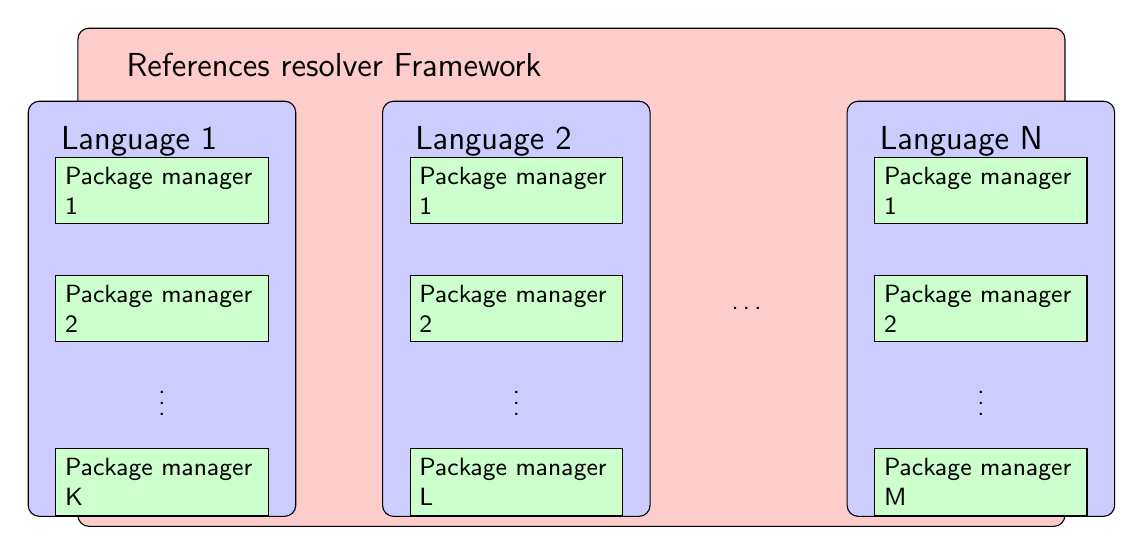
\begin{tikzpicture}
\node (rr) [framework] {};
\node [xshift=+5mm, yshift=-2mm, below right] at (rr.north west) {\large References resolver Framework };


\node (lang1) at ([xshift=-52mm,yshift=-4mm]rr) [lang] {};
\node [xshift=+3mm, yshift=-2mm, below right] at (lang1.north west) {\large Language 1 };
\node (lang2) at ([xshift=-7mm,yshift=-4mm]rr) [lang] {};
\node [xshift=+3mm, yshift=-2mm, below right] at (lang2.north west) {\large Language 2 };
\node (langn) at ([xshift=+52mm,yshift=-4mm]rr) [lang] {};
\node [xshift=+3mm, yshift=-2mm, below right] at (langn.north west) {\large Language N };
\node at ($(lang2)!.5!(langn)$) {\ldots};

\node (l1pm1) at ([yshift=+15mm]lang1) [entry] {Package manager 1};
\node (l1pm2) at ([yshift=0mm]lang1) [entry] {Package manager 2};
\node (l1pmn) at ([yshift=-22mm]lang1) [entry] {Package manager K};
\node at ($(l1pm2)!.5!(l1pmn)$) {\vdots};

\node (l2pm1) at ([yshift=+15mm]lang2) [entry] {Package manager 1};
\node (l2pm2) at ([yshift=0mm]lang2) [entry] {Package manager 2};
\node (l2pmn) at ([yshift=-22mm]lang2) [entry] {Package manager L};
\node at ($(l2pm2)!.5!(l2pmn)$) {\vdots};

\node (lnpm1) at ([yshift=+15mm]langn) [entry] {Package manager 1};
\node (lnpm2) at ([yshift=0mm]langn) [entry] {Package manager 2};
\node (lnpmn) at ([yshift=-22mm]langn) [entry] {Package manager M};
\node at ($(lnpm2)!.5!(lnpmn)$) {\vdots};


\end{tikzpicture} 
\caption{Example scheme representing several languages and package managers} 	\label{fig:lang_pm}
\end{figure}
\subsection*{Encapsulation of CSARs with extarnal Packages}\label{subs:encaps}
Here will be defined some methods of encapsulation of a CSAR containing external packages.
%It will be defined two methods  which install external packages during the deployment.
%The encapsulation must be achieved through the download of external packages and generation of a new TOSCA node for each of them. 
%But it can be interesting to analyze other techniques to encapsulate a CSAR. 
At first, one will describe the $generate$ $custom$ $repositories$ and $generate$ $shared$ $repositories$ methods not representing packages in a TOSCA topology and then the $one$ $node$ $for$ $one$ $package$ and $sets$ $of$ $packages$ methods mirroring packages into the topology.
\subsubsection*{Generate Custom Repositories}
It's possible to download all necessary packages and create one's own custom package repository for each operating system used in the application. 
Then one must rework any package installation commands or exchange system preferences to setup an access to the custom repository.
This method introduces minimal changes into a structure of TOSCA application.
The main problem is the creation of the custom repositories. 
When a TOSCA application consists of many operating systems executing on devices with limited capabilities, it may be difficult to start custom repositories on each of them.
\subsubsection*{Generate Shared Repository}
Another opportunity is to create a single repository for all operating systems in a TOSCA application.
It can be difficult to choose the right location for such a server, but since the applications often represents connected systems, this step can redistribute the load to a more powerful device.
It is difficult to estimate the changes which will occur in a TOSCA topology while applying such a method.
\subsubsection*{One Node for One Package}
%This method was suggested by the \gls{uniiaas}. 
A new TOSCA node will be created for each downloaded package. 
All dependencies between packages will be mirrored to a TOSCA topology.
This is a very visual method, facilitating the understanding of dependencies between packages.
\subsubsection*{Sets of Packages} \label{mode:setsofpkg}
The set of depended packages from a dependencies tree related to an external reference can be combined and represented in a TOSCA topology as a single node.
An installation of such a node will lead to the installation of all needed packages.
This way a small size of a TOSCA application's structure will be achieved.
It will be impossible to trace dependencies (since many packages are represented by one node), but it can help to avoid a difficult structure which consists of hundreds of nodes. 

\subsection{Encapsulation of CSARs with extarnal files}
%At the startup of the software, a user will be able to choose modes of operation.
%It was developed the concepts for two modes for external references presented by package installations and two modes for external references presented by file downloads.
%The default mode for package processing is the "one node for one package" mode. 
%In this mode, a new TOSCA node will be created for each used package from a packages database and dependencies between packages from the database will be mirrored to a TOSCA topology.
%Besides the default mode of operation, the "sets of packages" mode described in section~\ref{mode:setsofpkg} will be developed to provide possibility to generate relatively small encapsulated applications.
%This mode will be called the single node mode.
%To create the sets properly, the language module must combine the information about all packages needed for an artifact and then create a single TOSCA node for all of them.\\
It was developed two modes to handle download commands in CSARs: $addition$ and $integration$.
They will be presented shortly.

\subsubsection*{Addition}
The method is to add a new TOSCA node for each downloaded file.
This node will contain a deployment artifact presenting the downloaded file and an implementation artifact which will try to put the file into the right place.
Additionally a reference between the old node with an external reference and the added node must be created.

\subsubsection{Integration}
We can't be sure that the file added by the method described above will be available for other nodes.
Sometimes it can be difficult to get right position for the downloaded file. % outside the configuration manager.
We need to provide another opportunity for a user of the framework.
In the integration mode, the downloaded file must be integrated into the node which contain the file download command.
The command can be exchanged by a file move command to put the file into the right position.

\subsection{Representing Downloaded Packages in a TOSCA-Topology} \label{subs:repres}
Using some developed methods like Addition for external files or Sets of packages for external packages, downloaded data must be represented in the structure of a TOSCA Application.
We will introduce two new terms which can facilitate understanding: a package node and a file node.
These nodes denote to the defined and instantiated \gls{tosca} node, the purpose of which is to install packages or store files respectively.
Defined means, that the corresponding definitions of Node Type, Node Type Implementation, Artifact Types and Artifact Templates are integrated into the processed CSAR.
And to instantiate the nodes one need to create a Node Template.
The addition of new package and file nodes to the TOSCA topology can be divided into several steps.
\begin{itemize}
	\item One must add definitions for common elements like Artifact Types or Relationship Types. 
		This can be done once.
	\item The common definition of the created node will be represented by a Node Type.   
		It must contain the $install$ operation, which represents the capability to install the node.
		For the package nodes that will cause the installation of the package and the file move operation for the file nodes.
		%There will be described that this node must be installed.
	\item Artifacts (downloaded data and configuration files) will be referenced by Artifact Templates.
	\item A Node Type Implementation will combine the Artifact Templates to implement the $install$ operation.
	\item A Node Template will instantiate the node in the corresponding Service Templates.
		To determine the corresponding Service Template the author  uses the method described in section~\ref{subs:analyse}.
	\item A Reference Template will provide topology information allowing the observer (a user or a runtime environment) to determine dependencies between nodes.
		References will connect Node Templates contained external references and Node Templates resolving external references.
\end{itemize}
After an execution of these steps, the definition of a new TOSCA node will be finished and it can be used.

\subsection{Determining Architecture of the Final Platform} \label{finplatf}
To download the right instance of a package one must define its architecture.
But it is impossible to analyze the structure of any CSAR and determine the architecture of the device which the nodes will be deployed on.
There are many pitfalls here.\\
A single Service Template can use several physical devices with different architectures.
Many Node Types and Node Templates instantiated on different platforms can refer to the same Implementation Artifact.
This way one simple Implementation Artifact, for example with a bash script containing the "$apt$-$get$ $install$ $python$" command, can be executed by different Node Templates on different devices (for example with the arm, amd64 and i386 architectures) and will result in the download and installation of three different packages. 
For an end user, the ability to use such a simple command is a huge advantage, but for the framework, it can greatly complicate the analysis.
The following methods of architecture selection were designed.
\begin{itemize}
	\item $Deployment$ $environment$ $analysis$\\
	All  instances of packages for all supported architectures will be integrated into the processed CSAR. 
	The right instance will be chosen during deployment.
%	The script can analyze the system where it was started (for example using the "$uname$~$-a$" command) and depending on the result, it will install the package corresponding to the system's architecture.
	\item $Unified$ $architecture$\\
	The architecture will be defined for the whole CSAR.
	\item $Artifact$ $specific$ $architecture$\\
	The architecture will be defined for each artifact separately.
\end{itemize}
%\subsubsection*{Analysis of methods}
The $deployment$ $environment$ $analysis$, which at first sight seems to be the most reliable solution, brings many additional problems.
Packages for different platforms can differ not only by architecture but also by the version and the list of dependencies.
Chaos may occur when using methods mirroring dependencies between packages into a TOSCA topology.
The only found robust solution is to use an extended variant of the Sets of packages method described in section~\ref{mode:setsofpkg}. 
Using this method, all the data needed for installation of a package for one architecture will be stored in one set.
Framework must create a set of installation data for each supported architecture. 
The right set will be chosen during the deployment of the CSAR. %\\
The $artifact$ $specific$ $architecture$ method carries an additional complexity to the framework.
One must analyze each artifact and decide which architecture it will be executed on. 
This can be complicated by the fact that the same artifact can be executed on different architectures. %\\
The $unified$ $architecture$ method was chosen as the simplest and easiest to implement.
If it will be necessary, this method can easily be expanded to $artifact$ $specific$ $architectures$ or to $deployment$ $environment$ $analysis$.

%\subsection{Extensibility}
%The framework should handle different languages, each of them can support various package managers.
%An language module should filter files not belonging to the language, accepted files will be processed 
%This principle can be illustrated by a Figure \ref{fig:lang_pm}.
%% !TeX spellcheck = en_US

% We need layers to draw the block diagram
\usetikzlibrary{calc,positioning}

% Define a few styles and constants
\tikzstyle{entry}=[draw, fill=green!20, minimum height=2.5em]
\tikzstyle{ann} = [above, text width=5em]
\tikzstyle{framework} = [entry, text width=35em, fill=red!20, 
minimum height=18em, rounded corners]
\tikzstyle{lang} = [entry, text width=9em, fill=blue!20, 
minimum height=15em, rounded corners]
\def\blockdist{2.3}
\def\edgedist{2.5}

\begin{figure}
	\centering
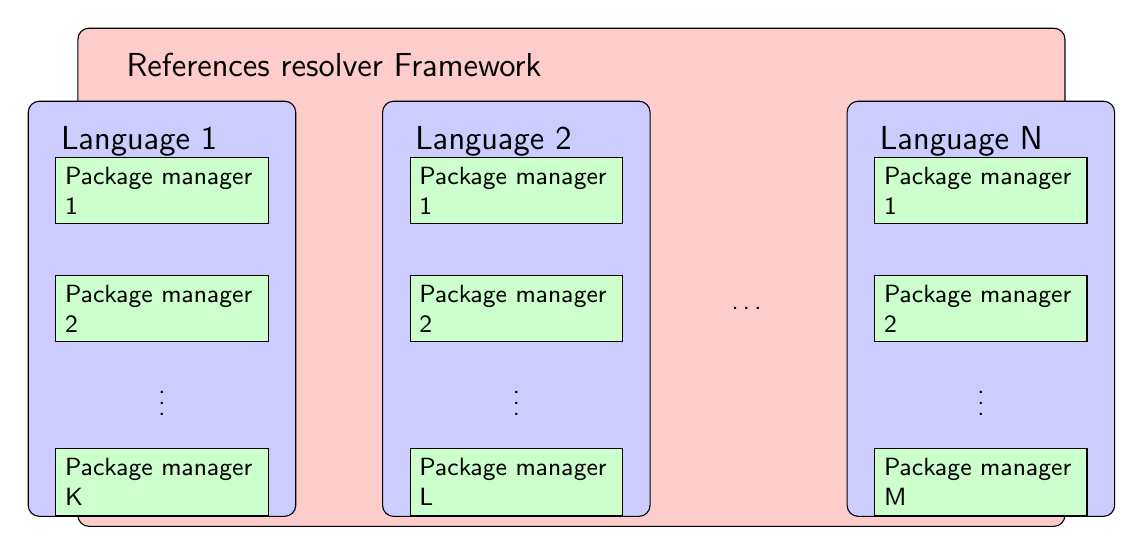
\begin{tikzpicture}
\node (rr) [framework] {};
\node [xshift=+5mm, yshift=-2mm, below right] at (rr.north west) {\large References resolver Framework };


\node (lang1) at ([xshift=-52mm,yshift=-4mm]rr) [lang] {};
\node [xshift=+3mm, yshift=-2mm, below right] at (lang1.north west) {\large Language 1 };
\node (lang2) at ([xshift=-7mm,yshift=-4mm]rr) [lang] {};
\node [xshift=+3mm, yshift=-2mm, below right] at (lang2.north west) {\large Language 2 };
\node (langn) at ([xshift=+52mm,yshift=-4mm]rr) [lang] {};
\node [xshift=+3mm, yshift=-2mm, below right] at (langn.north west) {\large Language N };
\node at ($(lang2)!.5!(langn)$) {\ldots};

\node (l1pm1) at ([yshift=+15mm]lang1) [entry] {Package manager 1};
\node (l1pm2) at ([yshift=0mm]lang1) [entry] {Package manager 2};
\node (l1pmn) at ([yshift=-22mm]lang1) [entry] {Package manager K};
\node at ($(l1pm2)!.5!(l1pmn)$) {\vdots};

\node (l2pm1) at ([yshift=+15mm]lang2) [entry] {Package manager 1};
\node (l2pm2) at ([yshift=0mm]lang2) [entry] {Package manager 2};
\node (l2pmn) at ([yshift=-22mm]lang2) [entry] {Package manager L};
\node at ($(l2pm2)!.5!(l2pmn)$) {\vdots};

\node (lnpm1) at ([yshift=+15mm]langn) [entry] {Package manager 1};
\node (lnpm2) at ([yshift=0mm]langn) [entry] {Package manager 2};
\node (lnpmn) at ([yshift=-22mm]langn) [entry] {Package manager M};
\node at ($(lnpm2)!.5!(lnpmn)$) {\vdots};


\end{tikzpicture} 
\caption{Example scheme representing several languages and package managers} 	\label{fig:lang_pm}
\end{figure}

%\subsection{Validation}
%Checking the output of the framework is an important stage in the development of the program.
%It is necessary to verify both the internal correctness of the output \gls{csar} and the possibility to deploy generated package nodes.
%The validity of internal dependencies can be checked by $Winery$ tool from OpenTOSCA.
%This tool allows create and edit CSAR archives and is also great for visualizing the results.
%Checking the deployment of the generated nodes can be done manually by entering commands which start the artifact's execution.


\section{Architecture}\label{sec:arch}
This section will present the architecture of the framework and the detailed description of its elements.
The main elements are a \boldmath $CSAR$ $handler$, a $references$ $resolver$, $language$ $modules$, $package$ $manager$ $modules$, $download$ $tool$ $modules$, a $package$ $handler$, and a $topology$ $handler$. \unboldmath

\subsection{CSAR handler} \label{subs:casr_h}
The CSAR handler provides an access to a \gls{csar} and maintains its consistency. 
It defines methods to process the metadata when adding new files, to \mbox{archive/unarchive} the CSAR, and to choose the final platform architecture. \\
The input CSAR is initially archived and must be decompressed in order to handle the content first.
When all external references will be resolved, the content will be archived to an output CSAR.
A new name-value pair must be added to the metadata for each new file integrated into the CSAR during processing. 
The name represents the internal path to the file and the value contains the type of the file. 
This type will be used by a runtime environment to choose the right behavior. %\\ %\\
As it was mentioned in section~\ref{finplatf}, the architecture of the final platform will be chosen for the entirely CSAR.
This can be done once at start.
%A command line interface must be provided for a user, to allow him to choose the architecture. 
The chosen architecture must be saved to the CSAR for the case of future processing by the framework to avoid the collisions between architectures of packages.

\subsection{References Resolver} \label{subs:RR}
References Resolver is the main element, whose execution is divided into three stages: $preprocessing$, $processing$, $finishing$. %\\
The first stage is the preprocessing.
CSAR is an archive file and it must be decompressed in order to manipulate the content. 
The CSAR handler can be used for this task.
As it was mentioned in section~\ref{subs:repres}, one need to add common definitions for used Artifact Types and References Types.
This will be done during the preprocessing stage.
Other important task is the generation of internal dependencies trees, which were described in section~\ref{subs:analyse}.
%During the $preprocessing$ stage, the CSAR will be unarchived, common definitions for Artifact Types and References Types added and internal dependencies trees generated.
%Figure \ref{fig:preproc} illustrates those steps.
After these operations starts the $processing$ stage.
During this stage all $language$ $modules$ will be activated.
Their operation is described in more detail in the next section. %\\
To finish the work all results will be packed into the output CSAR during the $finishing$ stage.
It's also necessary to update metadata of the CSAR to display the files added.
%% !TeX spellcheck = en_US

\usetikzlibrary{calc,arrows.meta,positioning,arrows}
\tikzset{
    every node/.style={font=\sffamily\small},
    main node/.style={shape=rectangle, rounded corners,
    	draw, align=center,
    	top color=white, bottom color=blue!20}
}

\tikzstyle{entry}=[draw, fill=green!20, minimum height=2.2em, text width=7em]
\tikzstyle{myentry}=[draw, fill=Dandelion!20, minimum height=2.5em, text width=7em]
\tikzstyle{ann} = [above, text width=5em]
\tikzstyle{frame} = [entry, text width=9em, fill=red!20, 
minimum height=17em, rounded corners]
\tikzstyle{csar_content} = [entry, text width=8em, fill=blue!20, 
minimum height=14em, rounded corners]
\def\blockdist{2.3}
\def\edgedist{2.5}
\begin{figure}
	\centering
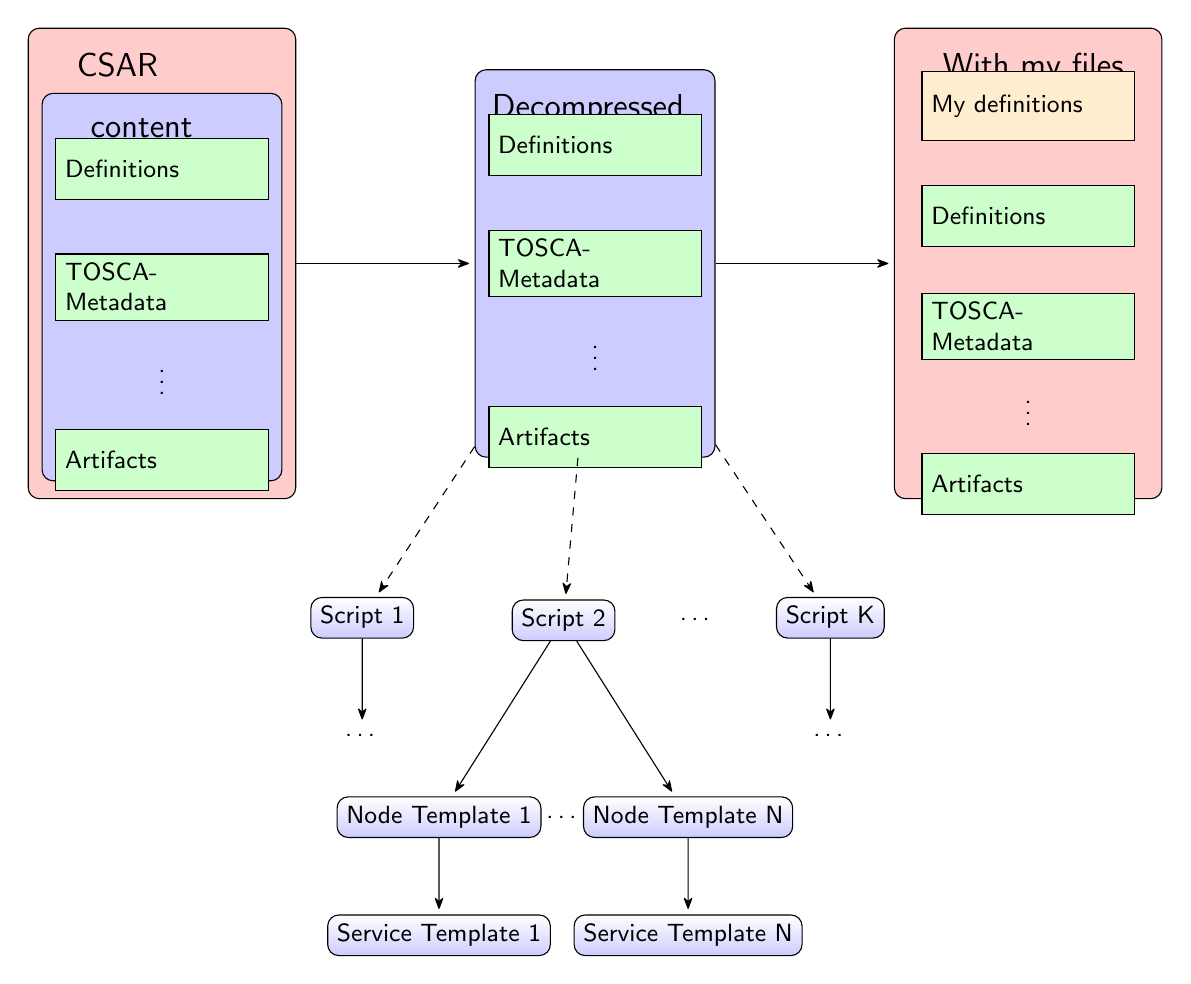
\begin{tikzpicture}[sibling distance=9em,->,>={Stealth[round,sep]},shorten >=1pt,auto,node distance=25mm]


\node (csar_frame) [frame] {};
\node [xshift=+5mm, yshift=-2mm, below right] at (csar_frame.north west) {\large CSAR};

\node (csar_content) at ( [yshift=-3mm]csar_frame) [csar_content] {};
\node [xshift=+5mm, yshift=-2mm, below right] at (csar_content.north west) {\large content};

\node (l2pm1) at ([yshift=+15mm]csar_content) [entry] {Definitions\\};
\node (l2pm2) at ([yshift=0mm]csar_content) [entry] {TOSCA-Metadata\\};
\node (l2pmn) at ([yshift=-22mm]csar_content) [entry] {Artifacts\\};
\node at ($(l2pm2)!.5!(l2pmn)$) {\vdots};
    
\node [right of=csar_frame, xshift=30mm](dc_frame) [csar_content] {};
\node [xshift=+1mm, yshift=-2mm, below right] at (dc_frame.north west) {\large Decompressed};
\draw [->] (csar_frame) -- (dc_frame);
\node (2pm1) at ([yshift=+15mm]dc_frame) [entry] {Definitions\\};
\node (2pm2) at ([yshift=0mm]dc_frame) [entry] {TOSCA-Metadata\\};
\node (2pmn) at ([yshift=-22mm]dc_frame) [entry] {Artifacts\\};
\node at ($(2pm2)!.5!(2pmn)$) {\vdots};

\node [right of=dc_frame, xshift=30mm](my_frame) [frame] {};
\node [xshift=+5mm, yshift=-2mm, below right] at (my_frame.north west) {\large With my files};
\draw [->] (dc_frame) -- (my_frame);
\node (3pmd) at ([yshift=+20mm]my_frame) [myentry] {My definitions\\};
\node (3pm1) at ([yshift=+6mm]my_frame) [entry] {Definitions\\};
\node (3pm2) at ([yshift=-8mm]my_frame) [entry] {TOSCA-Metadata\\};
\node (3pmn) at ([yshift=-28mm]my_frame) [entry] {Artifacts\\};
\node at ($(3pm2)!.5!(3pmn)$) {\vdots};


\node[below=of dc_frame,main node, node distance=10mm, xshift=-4mm, yshift=+7mm] (11) {Script 2}
child { node[main node, yshift=-10mm]  (n21) {Node Template 1} 
		child { node[main node] (s31) {Service Template 1}}  
}
child { node[main node, yshift=-10mm]  (n22) {Node Template N} 
	child { node[main node] (s32) {Service Template N}}  
};
\draw [dashed,->] (dc_frame) -- (11);
\node[below left=of dc_frame,main node,xshift=+10mm] (12) {Script 1}
child { node  {\ldots} 
};
\draw [dashed,->] (dc_frame) -- (12);
\node[below right=of dc_frame,main node, xshift=-10mm] (13) {Script K}
child { node  {\ldots} 
};
\draw [dashed,->] (dc_frame) -- (13);
\node at ($(11)!.5!(13)$) {\ldots};
\node at ($(n21)!.5!(n22)$) {\ldots};

\end{tikzpicture} 
\caption{Preprocessing: decompression, adding files and generating dependencies} 	\label{fig:preproc}
\end{figure}

\subsubsection{Language Modules} \label{subs:archlm}
Each $language$ $module$ describes a handling of one language used to write configuration files.
This module must accept only the files written in the language.
It also contains a list of supported package manager modules and download tool modules.
Each language module must provide the capability for the given package to generate a TOSCA node which must use the language to install the package.
For example a Bash module must provide capability to define new package nodes which use Bash to install the packages.
This means that a configuration file and definitions for Artifact Templates, a Node Type, and a Node Type Implementation should be created by a language module.\\
As it was already mentioned above,a language module analyzes all files one by one and checks their belonging to the language during the $processing$ stage. 
Any files not belonging to the described language are filtered out.
The remaining files are transferred to the language module's $package$ $manager$ $modules$ and $download$ $tool$ $modules$.
%For example, a $bash$ module will pass only files with $".sh"$ extension which start with the $"\#!/bin/bash"$ line.
Some modules can have an additional functionality.
For example an $ansible$ module should provide capability to unpack zip archives where ansible playbooks can be stored.
%Since ansible playbooks don't contain a specific header or marker, the single sign of ansible files is the "$.yml$" extension. 
%In the single node mode it will collect names of required packages from the corresponding package manager modules and create a single TOSCA node for all of them.

\subsubsection{Package Manager Modules} \label{subs:archpmm}
These modules process specified package managers.
They are integrated into language modules and become from them files to analyze.
To identify an external reference a package manager module will parse the given files. 
They must identify package installation commands which use the handled package manager.
Package manager modules find external references, remove them and transmit the package names to the $package$ $handler$ which is described in section~\ref{subs:archph} and returns the list of all required packages back to the package manager module which will transfer them farther back to a language module.
Figure~\ref{fig:lang_ph} illustrates data flow between language modules, package manager modules and the package handler.\\
An example will be provided for the $apt$-$get$ module for the Bash language.
The $apt$-$get$ package manager was described in section~\ref{subs:depapt}.
The module will read the given file line-by-line searching for the commands starting with the "apt-get install" string.
Such commands use the $apt$-$get$ package manager to install packages from external sources and must be removed from the file.
The arguments of this command is the list of package names which need to be installed.
These names must be transferred to the package handler.
%Such commands must be commented out and their arguments should be divided into separate package names which will be transferred to the package handler. 
% !TeX spellcheck = en_US
\usetikzlibrary{calc,arrows.meta,positioning}
\tikzset{
    every node/.style={font=\sffamily\small},
    main node/.style={shape=rectangle, rounded corners,
    	draw, align=center,
    	top color=white, bottom color=blue!20},
    data node/.style={shape=rectangle,
    draw, align=center,
    top color=white, bottom color=red!20}
}

\begin{figure}
	\centering
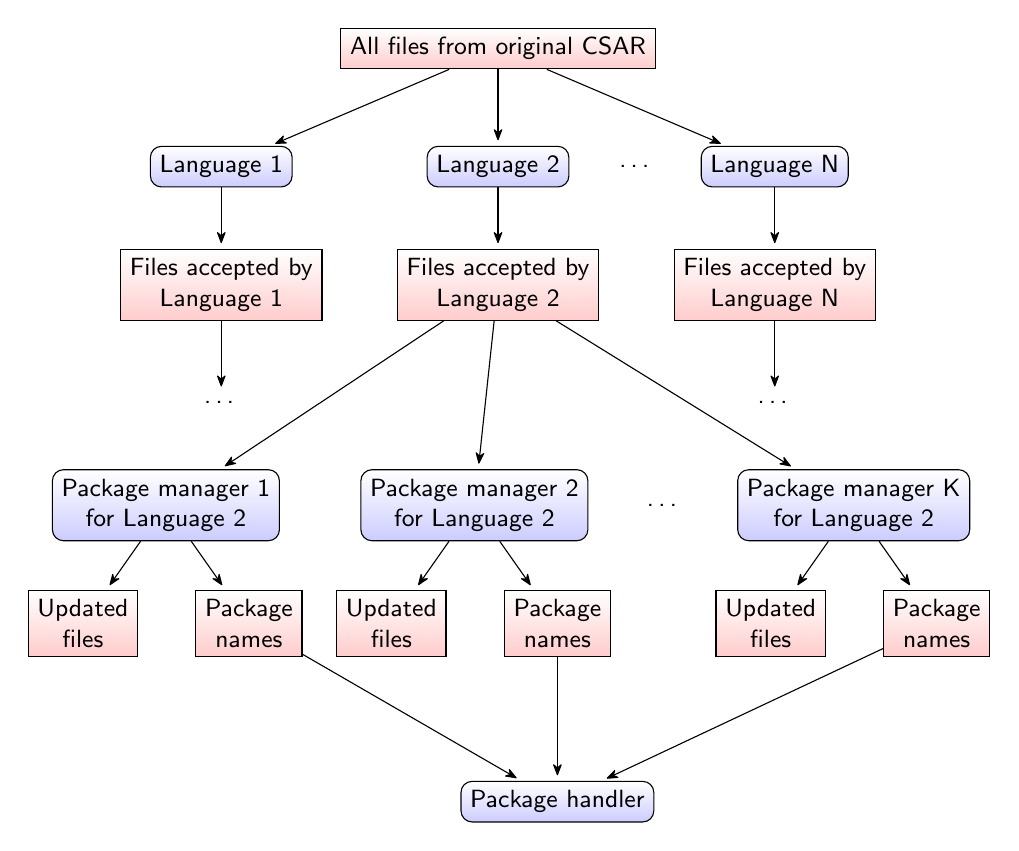
\begin{tikzpicture}[->,>={Stealth[round,sep]},shorten >=1pt,auto,level 1/.style={sibling distance=10em,node distance=25mm},
level 2/.style={sibling distance=8em,node distance=30mm},
level 3/.style={sibling distance=12em,node distance=30mm},
level 4/.style={sibling distance=6em,node distance=25mm},
level 5/.style={sibling distance=8em,node distance=25mm},
level 6/.style={sibling distance=8em,node distance=25mm}]
    \node[data node] (1)  {All files from original CSAR}
    child { node[main node](2) {Language 1} 
    	child { node[data node](21) {Files accepted by\\ Language 1} 
    		child { node {\ldots}}}}
	child { node[main node] (3) {Language 2}
		child { node[data node](31) {Files accepted by\\ Language 2} 
			child { node[main node, yshift=-13mm](32) {Package manager 1\\for Language 2} 
				child { node[data node](36) {Updated\\ files}}
				child { node[data node](37) {Package\\ names}}}
			child { node[main node, yshift=-13mm, xshift=-3mm](33) {Package manager 2\\for Language 2}
				child { node[data node](34) {Updated\\ files}}
				child { node[data node](35) {Package\\ names}}}
			child { node[main node, yshift=-13mm, xshift=+3mm](34) {Package manager K\\for Language 2}
				child { node[data node](38) {Updated\\ files}}
				child { node[data node](39) {Package\\ names}}}
			}
		}
    child { node[main node] (4) {Language N}
    	child { node[data node](41) {Files accepted by\\ Language N} 
    		child { node {\ldots}}}}
	;

	\node [main node,below, yshift=-20mm] at (35) (ph) {Package handler};
    \node at ($(3)!.5!(4)$) {\ldots};
    \node at ($(33)!.5!(34)$) {\ldots};
    \draw [->] (35) --(ph);
    \draw [->] (37) --(ph);
    \draw [->] (39) --(ph);
    
\end{tikzpicture} 
\caption{Data flow scheme between language modules, package manager modules and package handler.} 	\label{fig:lang_ph}
\end{figure}

\subsubsection{Download Tool Modules}
Each download tool module process the defined data download tool.
It analysis the files provided by a language module which it was defined in.
Identified external references must be resolved by removing installation commands, downloading files and integrating them into the processed CSAR.
Behavior features will be defined by the selected operation mode.

\subsection{Package Handler} \label{subs:archph}
The $package$ $handler$ provides interface to communicate with an operating system's package manager. 
It can download installation data, determine the type of dependency between packages and provide a list with dependent packages for the given package. \\
To download the installation data this component will use the given package name and the architecture specified by the CSAR handler.
Then it transfers the package name to the $topology$ $handler$ and repeats these actions for all depended packages recursively. 
During the process it stores all names of packages from the dependencies tree of original package and sends them back to the calling package manager module.
If the $apt$-$get$ package manager is used  the command "$apt$-$get$ $download$ \textbf{package}" can be used to download the data. 
The architecture can be specified by a ":$architecture$" suffix, for example, a "$package$:$arm$" mean the package for the $arm$ architecture.
The list of dependencies will be obtained using an operating system package analyzer. % the "apt-cache depends \textbf{package}" command. 
Its output should be parsed in order to extract the names of depended packages.
Type of dependency can be achieved in the same manner.
Of course, in case of a fault during a download of a package, a user interface should be provided to find a solution.
For example it can be: retry the download, ignore the package, rename the package or even break the framework's execution.

\subsection{Topology Handler} \label{subs:archtop}
%This element should handle the TOSCA topology and it has two main tasks: to analyze the TOSCA topology during the preprocessing stage to create internal dependencies trees and to use those trees to create TOSCA definitions for Node Templates and Relationship Templates in the right places for the packages provided by the package handler.
This element handles the TOSCA topology and it has two main tasks: create internal dependencies trees and generate TOSCA definitions for packages provided by the package handler.
To build the trees the analysis of the TOSCA topology will be used during the preprocessing stage.
This procedure was described in section~\ref{subs:analyse}.
The needed definitions for instantiation of a new TOSCA node include Node Templates and Relationship Templates which were described in section~\ref{subs:repres}.
To create the definitions in the right places the generated internal dependencies trees will be used.
The internal dependencies trees must be updated to represent changes after addition of new Node Templates and Relationship Templates.
%$Topology$ $handler$ adds a package to the topology. 
%This includes adding new files and updating existing files. 
%Necessary steps were described in section \ref{subs:repres}.